%COPYRIGHT PAGE%-
\thispagestyle{empty}
\begin{center}
\includegraphics[scale=0.35]{RITESbuilding1.jpg} %logo}
\end{center}

%~\vfill
\vskip 2cm

\noindent 

\begin{center}
\begin{tikzpicture}    % Now typeset a sample box.
\node[text width=.5\textwidth,   fill=yellow!30,   fill opacity=0.6,  text opacity=0.8,   	%but this also makes photo transparent
      inner sep=10pt]{	 \centering {\bf\Large A Government of India Compnay \\ under Ministry of Railways}\\
      Chittaranjan Locomotive Works \\
\vskip 0.3cm   
   \includegraphics[width=0.5\textwidth]{RITESlogo} \\
\vskip 0.4cm
}; %Photo insertion credit: gopalkumar@rites.com   };
\end{tikzpicture}

\end{center}


\vfill

%\AddToShipoutPicture*{ \put(150,50){  \includegraphics[scale=0.24]{RITESlogo.png}  } } % bottom Image background


\begin{center}
%\colorbox{white}{\EANisbn[SC4]}
\includegraphics[scale=0.551]{img/gkqrcode.jpg}

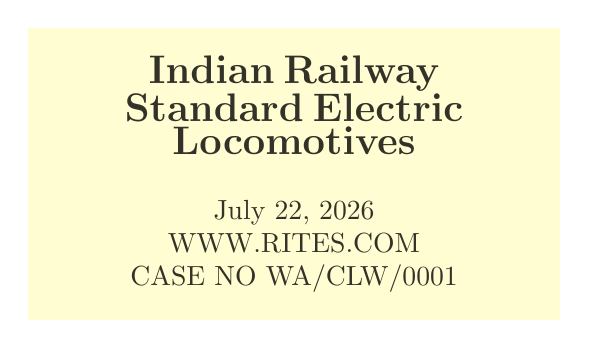
\begin{tikzpicture}    % Now typeset a sample box.
\node[text width=.5\textwidth,   fill=yellow!30,   fill opacity=0.6,  text opacity=0.8,   inner sep=10pt]  	%but this also makes photo transparent
    {	 \centering {\bf\Large Indian Railway Standard Electric Locomotives}\\
\vskip 0.4cm
\today \\
WWW.RITES.COM\\
CASE NO WA/CLW/0001\\
};
\end{tikzpicture}

\vspace*{\baselineskip}

\textbf{\textcolor{red!80}{Expotech Division, RITES Limited \texttt{http://www.rites.com}}}
\vspace*{\baselineskip}

\colorbox{white}{
\textbf{\textcolor{red!60}{Cover Illustration: Indian Railway Locomotives  \textbullet\ \texttt{http://www.rites.com}}}   }
\end{center}


\noindent Copyright \copyright\ RITES Ltd 2016\\ % Copyright notice

\noindent \textsc{Expotech Division}\\ % Publisher

\noindent \textsc{www.rites.com}\\ % URL

\noindent This offer is prepared for the specific use of RITES prospective clients to enable technical and commercial evaluation of the offer submitted by RITES.
For any clarification, please contact gopalkumar@rites.com  \url{http://www.rites.com}.\\ % License information

\noindent \textit{ \today} % Printing/edition date

